\section{Java}

\begin{defi}{CGI}
    \emph{Common Gateway Interface (CGI)} dient als Schnittstelle, um externe Programme auszuführen.
    Jede Anfrage erzeugt einen eigenen Prozess.
    Es ist ein Sprach- bzw. System-unabhängiges Konzept.
\end{defi}

\begin{defi}{Servlet-Engine}
    Die Servlet-Engine enthält und verwaltet die Servlets über ihren gesamten Lebenszyklus.

    Sie bindet die Servlets über feste vorgegeben Interfaces ein und stellt die Dienste zum Empfangen von Anfragen und Senden von Antworten bereit.

    Somit bildet sie die Kommunikationsendpunkte für die Servlets, die über HTTP-URLs angesprochen werden können
\end{defi}

\begin{defi}{Servlet}
    Ein \emph{Servlet} ist eine abgeleitete Java-Klasse, die von einem Container verwaltet wird und dynamische HTML-Inhalte generiert.

    Servlets haben keine main-Methode.
    Die Programmtechnische Nutzung wird durch die Servlet-API gesteuert:
    \begin{itemize}
        \item \texttt{init}
        \item \texttt{service} oder \texttt{doGet} bzw. \texttt{doPost}
        \item \texttt{destroy}
    \end{itemize}

    Sie sind dauerhafte Prozesse, die zumeist auch über Anfragen hinweg existieren.
    Mehrere Anfragen existieren in der gleichen Instanz.

    Ein spezifisches Servlet unterliegt einem genau festgelegten Lebenszyklus:
    \begin{enumerate}
        \item Laden der Servlet-Klasse und instanziieren (on demand)
        \item Initialisieren des Servlet-Objekts
        \item Verarbeitung der verschiedenen Anfragen
        \item Entfernen des Servlet-Objekts
        \item Entladen der Servlet-Klasse
    \end{enumerate}

    Intern stehen drei Umgebungsvariablen zur Verfügung:
    \begin{itemize}
        \item \texttt{PATH\_INFO} bzw. \texttt{req.getPathInfo();}
        \item \texttt{REMOTE\_HOST} bzw. \texttt{req.getRemoteHost();}
        \item \texttt{QUERY\_STRING} bzw. \texttt{req.getQueryString();}
    \end{itemize}
\end{defi}

\begin{example}{Servlet}
    \begin{lstlisting}[language=Java]
        import java.io.*;
        import javax.servlet.*;
        import javax.servlet.http.*;

        public class PokemonServlet extends HttpServlet {
            public void init() { ... }
            public void destroy() { ... }

            public void doGet(HttpServletRequest req, HttpServletResponse res)
                throws IOException, ServletException {
                res.setContentType("text/html");
                PrintWriter out = response.getWriter();

                // Beispiel cookie
                Cookie cookie = new Cookie("lieblings_pokemon", "Glumanda");
                res.addCookie(cookie);

                // Beispiel session
                HttpSession session = request.getSession();
                session.setAttribute("lieblings_pokemon", "Glumanda");
                
                out.println(
                    "<html>\n" +
                    "<head>\n" +
                    "<title> Pokemon </title>\n" +
                    "</head>\n" +
                    "<body> Glumanda [4] </body>\n" +
                    "</html>\n"
                )
            }
        }
    \end{lstlisting}
\end{example}

\begin{defi}{Tomcat}
    \emph{Tomcat} ist eine vollständig in Java geschriebene open Source Referenzimplementierung der Apache Foundation der Servlet API.
    Es dient als leicht-gewichtiger Servlet-Container, der z.B. keine Enterprise Java Beans unterstützt.
\end{defi}

\begin{defi}{JSP}
    \emph{Java Server Pages (JSP)} kehrt die Servlet Idee \enquote{Java-Code generiert HTML} um: \enquote{HTML-Seiten beinhalten Java-Code}.
    Die Anweisungen werden durch spezielle Tags gekennzeichnet.

    JSP-Seiten werden automatisch in Servlets übersetzt.
\end{defi}

\begin{example}{JSP}
    \begin{lstlisting}[language=Java]
        <%@ page contentType="text/html"%>
        <!DOCTYPE html>
        <html>
        <head> <title> Pokemon </title> </head>
        <body>
            <p> <%= String.toUpperCase("Glumanda"); %> </p>
            <% out.println("Glumanda > Bisasam!"); %>
        </body>
        </html>
    \end{lstlisting}
\end{example}

\begin{bonus}{Elemente JSP}
    Es gibt neben den HTML-Elementen drei wichtige JSP-Konstrukte:
    \begin{itemize}
        \item Scripting-Elemente bzw Java-Fragmente

              lokale Variablen sind:
              \begin{itemize}
                  \item \texttt{pageContent}: Zugriff auf Objekte in den verschiedenen Gültigkeitsbereichen
                  \item \texttt{HttpServletRequest}
                  \item \texttt{session}: sitzungsorientierte Anwendung
                  \item \texttt{out}: Ausgabe
              \end{itemize}
        \item Direktiven, die die Gesamtstruktur des Servlets kontrollieren

              Es gibt drei Arten von Direktiven:
              \begin{itemize}
                  \item page: zum Importieren einer Klasse
                  \item include: Fügt eine weitere JSP-Datei ein
                  \item taglib: zum Einführen eigener JSP-Tags
              \end{itemize}
        \item Aktionen bzw. Funktionalitäten zur Laufzeit, die das Servlet beeinflussen

              z. B.:
              \begin{itemize}
                  \item Include: Einfügen einer HTML- oder JSP-Seite zur Laufzeit
                  \item Forward: Anfragen und Antwort werden an eine andere JSP-Seite übergeben
              \end{itemize}
    \end{itemize}
\end{bonus}

\begin{defi}{Model View Controller (Prinzip)}
    \begin{itemize}
        \item Model-Objekt
              \begin{itemize}
                  \item definiert die Datenstruktur der Anwendung
                  \item speichert die Daten
                  \item stellt Methoden zur Änderung der Daten zur Verfügung
                  \item Realisiert manchmal die Geschäftslogik
              \end{itemize}
        \item View-Objekt
              \begin{itemize}
                  \item stellt die Bildschirmpräsentation dar
                  \item Objekt erhält die Daten vom Model
                  \item Benutzender führt auf der View die Aktion aus
                  \item die Aktionen werden durch den Controller an das Model weitergeleitet
              \end{itemize}
        \item Controller-Objekt
              \begin{itemize}
                  \item Reaktion und Verarbeitung von Benutzungseingaben
                  \item Vermittler zwischen Model und View
                  \item Realisiert oftmals die Geschäftslogik
              \end{itemize}
    \end{itemize}
\end{defi}

\begin{defi}{Model View Controller (Implementierung)}
    \begin{center}
        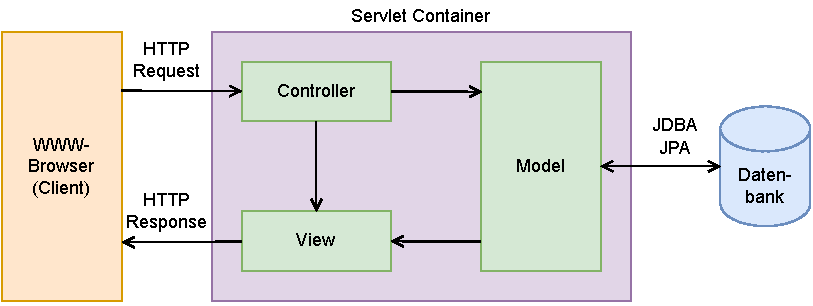
\includegraphics[width=0.75\textwidth]{includes/figures/defi_model_view_controller.pdf}
    \end{center}

    \begin{itemize}
        \item Model
              \begin{itemize}
                  \item Realisation zumeist mittels Java Beans
                  \item Java Beans enthalten die eigentliche Programmlogik
                  \item Java Beans berechnen die Ergebnisse und speichern Zustände
                  \item Java Beans sind unabhängig von der Webschnittstelle
              \end{itemize}
        \item View
              \begin{itemize}
                  \item Nutzung von JSP-Seiten
                  \item Anzeige der Ergebnisse
                  \item Ziel: Möglichst wenig Java Code
              \end{itemize}
        \item Controller
              \begin{itemize}
                  \item Programmieren eines Servlets
                  \item Einlesen und Überprüfen der übergeben Parameter
                  \item Aufrufen der eigentlichen Programmlogik im Model
                  \item Weitergabe des Ergebnisses an die passende View
              \end{itemize}
    \end{itemize}
\end{defi}

\begin{defi}{Java Beans}
    Enterprise Java Beans [\ldots] are meant to perform server side operations, such as executing complex algorithms or performing highly transactional business operations.
    Server components need to run in a highly available, fault tolerant, transactional, mutli-user, secure environment.
    The application server provides sich a server side environment for the enterprise beans\ldots
    Typically, EJB components can perform any of the following tasks:
    \begin{itemize}
        \item Perform business logic
        \item Access a database
        \item Integrate with other systems
    \end{itemize}
\end{defi}